% Generated by code/analysis/make_paper_figures.py; edit that source for tables.
\section{Verified pilot measurements}
\label{app:pilot-details}
The values below are reductions of \texttt{doc/auto/initial-phase-results.json},
independently checked against saved predictions and state arrays before this manuscript.
Each cell has one training seed (0), 1,500 optimization steps and 256 paired
evaluation episodes per horizon. Checkpoints minimize the same balanced validation loss:
step 300 for both categorical cells, 400 for continuous GRU and 200 for continuous LSTM.
Each cue-conditioned cloud fixes the complete driver and terminal phase, with 512
training histories and 256 held-out probe histories. The GRU state has 128 coordinates;
the LSTM concatenates all 128 hidden and 128 cell coordinates. Clouds, coordinates and
horizons are not independent training replicates. No confidence interval is inferred
from their spread. The query readout uses the model's native hidden state.

\subsection{Native task behavior}
Both categorical models have identical aggregate accuracies in both arms:
5.46875\%, 6.25\% and 5.078125\% at $R=1,2,16$, respectively.
The uniform-classifier reference is 6.25\%. Their paired error contrasts and
$\DID$ are exactly zero in the saved evaluation samples. All four models fail
the original engineering criterion at $R=1$ and $R=2$: accuracy at least 25\%
or continuous MSE at most 0.25 in both arms. Failure therefore precedes the
stronger competence requirements of the proposed confirmatory design.

\begin{table}[htbp]
\centering\small
\caption{Continuous native MSE, computed on paired evaluation episodes. The zero predictor uses the exact same saved targets. Values are rounded for display; contrasts use full-precision reductions.}
\label{tab:pilot-native}
\begin{tabular}{llrrr}
\toprule
Model & $R$ & Periodic & Matched control & Zero predictor \\
\midrule
GRU & 1 & 0.352933567 & 0.352933567 & 0.353299860 \\
GRU & 2 & 0.364228713 & 0.364228594 & 0.359106231 \\
GRU & 16 & 0.333522172 & 0.333522153 & 0.334111881 \\
LSTM & 1 & 0.352472891 & 0.352472891 & 0.353299860 \\
LSTM & 2 & 0.365605069 & 0.365604997 & 0.359106231 \\
LSTM & 16 & 0.334947432 & 0.334947418 & 0.334111881 \\
\bottomrule
\end{tabular}
\end{table}

The continuous periodic-minus-control differences at $R=2$ are
$1.19058\times10^{-7}$ (GRU) and $7.25557\times10^{-8}$ (LSTM);
at $R=16$ they are $1.91821\times10^{-8}$ and $1.34424\times10^{-8}$.
Their corresponding $\DID$ values are $-9.98763\times10^{-8}$ and
$-5.91133\times10^{-8}$. These seed-0 differences neither establish a
periodicity effect nor equivalence in competent models.

\subsection{Cue-conditioned probes and geometry}
Tables~\ref{tab:cloud-gru-categorical}--\ref{tab:cloud-lstm-continuous} retain every
driver-panel/arm cloud separately. PR is participation ratio; $V=\tr C$ uses
sample-centered complete states and unbiased covariance. Probe columns report
the mean over the eight required cue coordinates of held-out accuracy (categorical)
or MSE (continuous), with training-label permutation as a control. The probes are
ridge fits with regularization 0.01 after training-cloud feature standardization.
$q$ is centered-state RMS divided by the RMS coordinate spacing of the stored
float32 states, a post hoc resolution diagnostic. It is not a numerical error bound
or a test of float64 dynamics. All displayed clouds have nonzero variance.

Every $R=2$ cloud has a real-label probe advantage over its shuffled-label
control. At $R=16$ this advantage is inconsistent. The feature-scale floor
of $10^{-8}$ can alter effective regularization across clouds and horizons;
floor-hit counts and independently re-reduced probe sensitivities are unavailable.
The observations therefore support residual short-horizon decodability in these
stored states, without establishing robust retention, native task use or a
long-horizon mechanism. The two categorical-LSTM $R=16$ control clouds have
511 distinct stored rows; each of the other clouds has 512. No geometry below
is interpreted as a Floquet spectrum or a causal memory estimate.

\begin{table}[htbp]
\centering\footnotesize
\caption{GRU categorical: all eight cue-conditioned clouds. P and C denote periodic and matched-control arms; panel IDs identify different fixed drivers. Probe metric: accuracy (\%).}
\label{tab:cloud-gru-categorical}
\begin{tabular}{lllrrrrr}
\toprule
$R$ & Panel & Arm & PR & $V$ & Real probe & Shuffled & $q$ \\
\midrule
2 & 0 & P & 2.534 & $5.926\!\times\!10^{-15}$ & 22.5098 & 6.2012 & 2.145 \\
2 & 0 & C & 2.446 & $5.944\!\times\!10^{-15}$ & 20.9473 & 6.3477 & 2.148 \\
2 & 1 & P & 2.530 & $5.479\!\times\!10^{-15}$ & 22.7539 & 6.0547 & 2.015 \\
2 & 1 & C & 2.536 & $5.454\!\times\!10^{-15}$ & 21.7285 & 7.1289 & 2.010 \\
16 & 0 & P & 31.267 & $1.377\!\times\!10^{-16}$ & 6.2012 & 5.7617 & 0.327 \\
16 & 0 & C & 29.496 & $1.213\!\times\!10^{-16}$ & 5.8105 & 5.6152 & 0.307 \\
16 & 1 & P & 33.585 & $1.134\!\times\!10^{-16}$ & 7.1289 & 5.1270 & 0.295 \\
16 & 1 & C & 30.683 & $1.086\!\times\!10^{-16}$ & 5.9082 & 6.0547 & 0.289 \\
\bottomrule
\end{tabular}
\end{table}

\begin{table}[htbp]
\centering\footnotesize
\caption{GRU continuous: all eight cue-conditioned clouds. P and C denote periodic and matched-control arms; panel IDs identify different fixed drivers. Probe metric: MSE.}
\label{tab:cloud-gru-continuous}
\begin{tabular}{lllrrrrr}
\toprule
$R$ & Panel & Arm & PR & $V$ & Real probe & Shuffled & $q$ \\
\midrule
2 & 0 & P & 1.103 & $7.347\!\times\!10^{-15}$ & 0.2342 & 0.3807 & 2.547 \\
2 & 0 & C & 1.107 & $7.298\!\times\!10^{-15}$ & 0.2346 & 0.3725 & 2.539 \\
2 & 1 & P & 1.105 & $7.350\!\times\!10^{-15}$ & 0.2409 & 0.3715 & 2.446 \\
2 & 1 & C & 1.098 & $7.601\!\times\!10^{-15}$ & 0.2404 & 0.3705 & 2.487 \\
16 & 0 & P & 24.847 & $1.109\!\times\!10^{-16}$ & 0.3655 & 0.3572 & 0.313 \\
16 & 0 & C & 22.876 & $1.351\!\times\!10^{-16}$ & 0.3597 & 0.3617 & 0.345 \\
16 & 1 & P & 26.093 & $7.864\!\times\!10^{-17}$ & 0.3343 & 0.3362 & 0.255 \\
16 & 1 & C & 20.737 & $1.399\!\times\!10^{-16}$ & 0.3387 & 0.3318 & 0.340 \\
\bottomrule
\end{tabular}
\end{table}

\begin{table}[htbp]
\centering\footnotesize
\caption{LSTM categorical: all eight cue-conditioned clouds. P and C denote periodic and matched-control arms; panel IDs identify different fixed drivers. Probe metric: accuracy (\%).}
\label{tab:cloud-lstm-categorical}
\begin{tabular}{lllrrrrr}
\toprule
$R$ & Panel & Arm & PR & $V$ & Real probe & Shuffled & $q$ \\
\midrule
2 & 0 & P & 24.077 & $3.086\!\times\!10^{-16}$ & 15.0879 & 6.0547 & 0.368 \\
2 & 0 & C & 24.274 & $4.535\!\times\!10^{-16}$ & 14.7461 & 6.7383 & 0.446 \\
2 & 1 & P & 18.232 & $4.288\!\times\!10^{-16}$ & 15.4297 & 6.0059 & 0.415 \\
2 & 1 & C & 19.896 & $4.798\!\times\!10^{-16}$ & 15.5273 & 6.7871 & 0.439 \\
16 & 0 & P & 11.429 & $2.765\!\times\!10^{-16}$ & 5.7129 & 4.9805 & 0.348 \\
16 & 0 & C & 27.260 & $2.537\!\times\!10^{-16}$ & 6.7383 & 5.5176 & 0.334 \\
16 & 1 & P & 24.249 & $2.305\!\times\!10^{-16}$ & 6.2012 & 5.9082 & 0.318 \\
16 & 1 & C & 25.590 & $1.862\!\times\!10^{-16}$ & 5.9082 & 7.0801 & 0.286 \\
\bottomrule
\end{tabular}
\end{table}

\begin{table}[htbp]
\centering\footnotesize
\caption{LSTM continuous: all eight cue-conditioned clouds. P and C denote periodic and matched-control arms; panel IDs identify different fixed drivers. Probe metric: MSE.}
\label{tab:cloud-lstm-continuous}
\begin{tabular}{lllrrrrr}
\toprule
$R$ & Panel & Arm & PR & $V$ & Real probe & Shuffled & $q$ \\
\midrule
2 & 0 & P & 6.640 & $5.657\!\times\!10^{-16}$ & 0.3180 & 0.3781 & 0.443 \\
2 & 0 & C & 7.028 & $6.284\!\times\!10^{-16}$ & 0.3163 & 0.3802 & 0.467 \\
2 & 1 & P & 6.628 & $5.180\!\times\!10^{-16}$ & 0.3100 & 0.3585 & 0.427 \\
2 & 1 & C & 6.770 & $5.991\!\times\!10^{-16}$ & 0.3030 & 0.3575 & 0.460 \\
16 & 0 & P & 22.329 & $1.935\!\times\!10^{-16}$ & 0.3634 & 0.3635 & 0.259 \\
16 & 0 & C & 19.777 & $2.000\!\times\!10^{-16}$ & 0.3644 & 0.3633 & 0.264 \\
16 & 1 & P & 18.987 & $2.429\!\times\!10^{-16}$ & 0.3429 & 0.3457 & 0.293 \\
16 & 1 & C & 20.487 & $1.779\!\times\!10^{-16}$ & 0.3398 & 0.3388 & 0.250 \\
\bottomrule
\end{tabular}
\end{table}

\subsection{An exact feature-scale counterexample}
\label{app:probe-scale}
The v1 probe uses $X^{\mathsf T}X+n\alpha I$ with $\alpha=0.01$ after
division by $\max(\operatorname{std}(h),f)$, where $f=10^{-8}$ and the
standard deviation uses divisor $n$. To isolate the resulting scale dependence,
let a scalar cue $u$ have zero mean and unit second moment in separate
deterministic training and test designs, and encode it as $h=au$, $a>0$.
Writing $r=a/\max(a,f)$, ridge predicts
$\widehat u=r^2u/(r^2+\alpha)$ and its test MSE is exactly
\begin{equation}
\label{eq:probe-floor}
\mathcal E_{\rm ridge}(a)=\left(\frac{\alpha}{r^2+\alpha}\right)^2.
\end{equation}
This error approaches the zero-predictor value as $a/f\to0$, although the
encoding stays invertible and the exact decoder $h/a$ retains the cue.
Without the floor, ridge error is $(\alpha/(1+\alpha))^2$ at every amplitude.
The figure script checks 101 amplitudes against the actual v1 probe, using
64 training and 257 distinct-design test points and float64 arithmetic.
This construction proves a diagnostic failure mode; it does not quantify its
contribution to the pilot probe contrasts or establish noise-robust memory.
\begin{figure}[htbp]
\centering
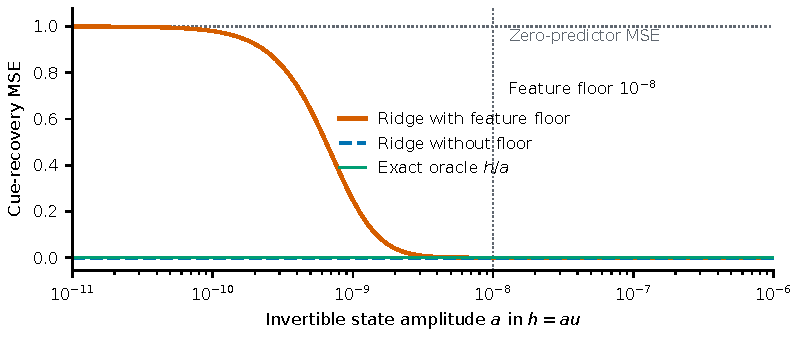
\includegraphics[width=0.82\linewidth]{figures/probe_scale_artifact.pdf}
\caption{A feature-standardization floor can manufacture probe deterioration under an invertible rescaling. The exact scalar construction has no noise or training failure. Orange is Eq.~\eqref{eq:probe-floor}, verified through the v1 ridge implementation; blue is floor-free ridge, with MSE $9.80\times10^{-5}$, and green is the exact inverse decoder, with zero mathematical error. These curves are analytic controls, not learned-model observations.}
\label{fig:probe-scale}
\end{figure}
